\documentclass{estilo}
\usepackage[spanish]{babel}
\usepackage{graphicx}
\usepackage{float}
\usepackage{amsmath}        % para los vectores columnas
\usepackage{amsfonts}       % para las negrita de pizarra
\usepackage{amssymb}        % para simbolos matematicos
\usepackage{hyperref}       % para utilizar referencias
\usepackage{multirow}       % para las tablas
\usepackage{dsfont}
\usepackage{listings}
\usepackage{xcolor}
\definecolor{codegreen}{rgb}{0,0.6,0}
\definecolor{codegray}{rgb}{0.5,0.5,0.5}
\definecolor{codepurple}{rgb}{0.58,0,0.82}
\definecolor{backcolour}{rgb}{0.95,0.95,0.92}
\lstdefinestyle{mystyle}{
    backgroundcolor=\color{backcolour},   
    commentstyle=\color{codegreen},
    keywordstyle=\color{magenta},
    numberstyle=\tiny\color{codegray},
    stringstyle=\color{codepurple},
    basicstyle=\ttfamily\footnotesize,
    breakatwhitespace=false,         
    breaklines=true,                 
    captionpos=b,                    
    keepspaces=true,                 
    numbers=left,                    
    numbersep=5pt,                  
    showspaces=false,                
    showstringspaces=false,
    showtabs=false,                  
    tabsize=2
}
\lstset{style=mystyle}

\usepackage{enumitem,multicol,setspace}
\newcounter{subenum}[enumi] % para las multicolumnas
\renewcommand{\thesubenum}{\arabic{subenum}}
\usepackage[nomessages]{fp}
\FPeval\thecolwidth{round(1/4:4)}% Specify number of columns -> column width
\newcommand{\newitem}[1]{%
  \refstepcounter{subenum}%
  \parbox{\dimexpr\thecolwidth\linewidth-.5\columnsep}{%
    \makebox[\labelwidth][r]{(\thesubenum)\hspace*{\labelsep}}%
    #1}\hfill%
}

\usepackage{scalerel,stackengine} % para el sombrero
\stackMath
\newcommand\rhat[1]{%
\savestack{\tmpbox}{\stretchto{%
  \scaleto{%
    \scalerel*[\widthof{\ensuremath{#1}}]{\kern-.6pt\bigwedge\kern-.6pt}%
    {\rule[-\textheight/2]{1ex}{\textheight}}%WIDTH-LIMITED BIG WEDGE
  }{\textheight}% 
}{0.5ex}}%
\stackon[1pt]{#1}{\tmpbox}%
}
\parskip 1ex

\usepackage{mathtools}      % floor y ceil
\DeclarePairedDelimiter\ceil{\lceil}{\rceil}
\DeclarePairedDelimiter\floor{\lfloor}{\rfloor} 

\usepackage[style=authoryear-comp]{biblatex}


\begin{document}
\maketitle

\justifying{
}

% \newpage
% \input{tex/consideraciones}
\newpage

\section{Problemas NP-Completos}

El problema consiste en encontrar el conjunto mínimo de jugadores que satisface los deseos de la prensa. Como datos de entrada tenemos los deseos de la prensa.


\subsection{Demostración que Hitting Set es un problema NP}

\subsubsection{Definición de problemas NP}
Los problemas NP son aquellos para los que existe un certificador eficiente, es decir, aquellos que se pueden validar en tiempo polinomial.

\subsubsection{Demostración}

\textbf{Introducción}

\hspace{0.5cm} Este problema consiste en determinar si, dado un conjunto \(A\) de \(n\) elementos, \(m\) subconjuntos \(B_1, B_2, ..., B_m\) de \(A\), y un número entero \(k\), existe un subconjunto \(C\) de \(A\) con \(|C| \leq k\) tal que \(C \cap B_i \neq \emptyset\) para cada \(i\) en el rango de \(1\) a \(m\), es decir, que exista al menos un elemento.

\hspace{0.5cm} La pertenencia a NP se demuestra que, dada una solución propuesta \(C\), es posible verificar en tiempo polinómico si cumple con las condiciones del problema. Esto implica verificar el tamaño de \(C\) para asegurarse de que \(|C| \leq k\), lo cual es un proceso polinómico, y verificar la intersección de \(C\) con cada \(B_i\), garantizando que \(C \cap B_i \neq \emptyset\) para cada \(i\), también en tiempo polinómico.

\newline
\newline

\textbf{Verificación}

\hspace{0.5cm} Tenemos dos condiciones que corroborar:


\begin{itemize}
    \item \textit{Tamaño del conjunto:} Verificar que $|C| \leq k$.
    \item \textit{Intersección con cada $B_i$:} Verificar que $C \cap B_i \neq \emptyset$ para cada $i$ en el rango de $1$ a $m$.
\end{itemize}

\hspace{0.5cm} Para la verificación del tamaño del conjunto, la operación de comparación $|C| \leq k$ toma $O(\log k)$ pasos, ya que el tamaño de $k$ se puede representar en $O(\log k)$ bits.

\hspace{0.5cm} Para la verificación de la intersección con cada $B_i$, se realiza una búsqueda o comparación de cada elemento de $C$ con los elementos de $B_i$. Dado que $|C| \leq k$ y $|B_i|$ está acotado por el tamaño de $A$, la verificación de cada intersección toma $O(k \cdot n)$ pasos.

\hspace{0.5cm} En total, el tiempo de verificación es de $O(\log k + k \cdot n)$, lo cual es polinómico. Por lo tanto, la verificación del Hitting-Set Problem toma tiempo polinómico y en consecuencia, el problema está en NP.


\subsection{Demostración que Hitting Set es un problema NP-Completo}

\subsubsection{Definición de problemas NP-completo}

\(X \in \text{NP-Completo}\) \(\Leftrightarrow\) \(X \in \text{NP} \land \forall Y \in \text{NP} (Y \leq_p X)\).

Esto quiere decir que: Sabemos que un problema es NP-Completo si y solo si es un problema que esta en NP y también sucede que para cualquier problema que esta en NP se puede reducir polinomialmente a el problema NP-Completo.

\newpage
\subsubsection{Demostración}

Utilizaremos el problema de la satisfacción booleana (SAT) como ejemplo de un problema NP-completo. Este problema plantea la pregunta de si, dado un conjunto de cláusulas, donde cada una es una combinación de variables booleanas conectadas por operadores OR, es posible encontrar una asignación de valores a las variables que satisfaga todas las cláusulas. Podemos reducir polinomicamente Hitting Set a SAT, hagamos la demostración:

Dada una instancia de SAT, construimos una fórmula booleana \(F\) para Hitting-Set Problem de la siguiente manera:

\begin{itemize}
    \item Cada variable en \(F\) se convierte en un conjunto en el conjunto universal \(X\).
    \item Cada cláusula en \(F\) se convierte en un subconjunto en \(B_i\).
\end{itemize}

Entonces, para resolver SAT, necesitamos encontrar un conjunto \(C\) tal que \(|C| \leq k\) y \(C \cap B_i \neq \emptyset\) para cada cláusula \(B_i\) en \(F\).

Supongamos que tenemos la siguiente instancia de SAT:

\[ F = (x_1 \lor x_2 \lor \neg x_3) \land (\neg x_1 \lor x_3) \land (\neg x_2 \lor \neg x_3) \]

Ahora, construimos la instancia correspondiente del \textit{Hitting-Set Problem} utilizando la reducción mencionada:

\begin{minipage}[t]{0.7\textwidth}
    \textbf{Conjunto universal:} \(X = \{x_1, x_2, x_3\}\).

    \vspace{0.5cm}

    \textbf{Subconjuntos \(B_i\):}
    \begin{align*}
        B_1 & = \{x_1, x_2, \neg x_3\} \\
        B_2 & = \{\neg x_1, x_3\} \\
        B_3 & = \{\neg x_2, \neg x_3\}
    \end{align*}
\end{minipage}
\hfill
\begin{minipage}[t]{0.3\textwidth}
    \begin{tikzpicture}[baseline=(current bounding box.north)]
        % Conjunto universal X
        \node[circle, draw] (x_1) at (0,0) {$x_1$};
        \node[circle, draw] (x_2) at (1,0) {$x_2$};
        \node[circle, draw] (x_3) at (2,0) {$x_3$};
        
        % Subconjuntos B_i
        \node[ellipse, draw] (B1) at (0.5,-1.5) {$B_1$};
        \node[ellipse, draw] (B2) at (1.5,-1.5) {$B_2$};
        \node[ellipse, draw] (B3) at (2.5,-1.5) {$B_3$};
        
        % Arrows
        \draw[->] (B1) -- (x_1);
        \draw[->] (B1) -- (x_2);
        \draw[->, red] (B1) -- (x_3);
        
        \draw[->, red] (B2) -- (x_1);
        \draw[->] (B2) -- (x_3);
        
        \draw[->, red] (B3) -- (x_2);
        \draw[->, red] (B3) -- (x_3);
    \end{tikzpicture}
\end{minipage}

Entonces, para resolver el \textit{Hitting-Set Problem}, necesitamos encontrar un conjunto de elementos seleccionados \(C\) tal que \(|C| \leq k\) y \(C \cap B_i \neq \emptyset\) para cada \(B_i\) en \(F\). Supongamos que \(k = 2\).

Un conjunto de elementos seleccionados posible podría ser \(C = \{x_1, \neg x_2\}\). Ahora verifiquemos que \(C\) es un conjunto de elementos seleccionados:

\begin{itemize}
    \item \textbf{Tamaño del conjunto:} \(|C| = 2 \leq 2\) (cumple con \(k\)).
    \item \textbf{Intersección con cada \(B_i\):}
        \begin{align*}
            C \cap B_1 & = \{x_1\} \neq \emptyset \\
            C \cap B_2 & = \{\neg x_2\} \neq \emptyset \\
            C \cap B_3 & = \emptyset \quad
        \end{align*}
\end{itemize}

Por lo tanto, \(C = \{x_1, \neg x_2\}\) es un conjunto de elementos seleccionados válido para la instancia del \textit{Hitting-Set Problem}, pero dado que SAT es un problema de decisión nos basta con saber que hay solución valida posible.

En resumen, hemos demostrado que el \textit{Hitting-Set Problem} está en NP y que es NP-completo al mostrar una reducción polinómica desde SAT.

\section{Algoritmo de Backtracking}

\subsection{Introducción}
El algoritmo consiste en explorar un espacio exponencial de soluciones al problema probando si agregando un jugador a la lista de jugadores convocados se logra satisfacer el Hitting Set Problem. Al ser esto una solución de fuerza bruta buscamos optimizar el algoritmo a través de varias condiciones de corte para evitar explorar soluciones que no resuelven el problema o son menos óptimas que una solución ya encontrada. 

Para asistir con estas optimizaciones decidimos representar el problema con una clase de manera que nos facilite guardar en el estado interno de la misma la mejor solución encontrada.

Se aplicaron las siguientes optimizaciones:
\begin{itemize}
\item{Como el algoritmo va probando las soluciones desde la menor cantidad de jugadores a la mayor pudimos hacer una optimización muy grande cortando la rama recursiva una vez que encontramos una solución menor a la almacenada para el problema (o cualquier solución valida en el caso de todavía no tener una).}

\item {Reducimos en cada llamado recursivo la lista de deseos con aquellos deseos que todavía quedan por satisfacer (excluyendo los deseos que ya tienen al menos un jugador que es parte de la solución actual)}

\item {Agregamos una lista con los jugadores descartados de manera que podamos detectar cuando algún deseo ya no se puede cumplir con los jugadores que quedan sin descartar.}

\end{itemize}

\subsection{Complejidad algorítmica}

La complejidad algorítmica es $O(2^n)$ ya que en el peor de los casos este algoritmo termina corriendo como su base de fuerza bruta, donde se prueban todas las combinaciones posibles de jugadores hasta encontrar una solución valida.

\newpage
\subsection{El algoritmo}
\begin{lstlisting}[language=Python]
def hitting_set_backtracking(deseos):
    return HittingSetBacktracking(deseos).buscar_solucion()

class HittingSetBacktracking():
    def __init__(self, deseos_prensa):
        self._solucion = None
        self._deseos_prensa = deseos_prensa
    
    def buscar_solucion(self):
        self._buscar_solucion(self._deseos_prensa, [], [])
        return list(self._solucion)

    def _buscar_solucion(self, deseos_pendientes, convocados, descartados):
        if not self._puede_ser_solucion_optima(convocados):
            return
            
        deseos_pendientes = _deseos_pendientes(deseos_pendientes, convocados)
        
        if not any(deseos_pendientes):
            self._marcar_mejor_solucion(convocados)
            return
    
        jugador = _jugador_siguiente(deseos_pendientes, descartados)
    
        if jugador == None:
            return
    
        if not _todos_los_deseos_se_pueden_cumplir(deseos_pendientes, descartados):
            return
                
        self._buscar_solucion(deseos_pendientes, convocados, [*descartados, jugador])
        self._buscar_solucion(deseos_pendientes, [*convocados, jugador], descartados)


    def _marcar_mejor_solucion(self, nueva_solucion):
        if self._puede_ser_solucion_optima(nueva_solucion):
            self._solucion = nueva_solucion
        
    def _puede_ser_solucion_optima(self, convocados):
        return not self._solucion or len(convocados) < len(self._solucion)

def _deseos_pendientes(deseos_prensa, convocados):
    deseos_restantes = []

    for deseo in deseos_prensa:
        cumplido = any(filter(lambda jugador: jugador in deseo, convocados))
        
        if not cumplido:
            deseos_restantes.append(deseo)
    
    return deseos_restantes

def _jugador_siguiente(deseos_pendientes, descartados):
    for deseo in deseos_pendientes:
        for jugador in deseo:
            if jugador in descartados:
                continue
            return jugador
    return None
    
def _todos_los_deseos_se_pueden_cumplir(deseos_prensa, descartados):
    for deseo in deseos_prensa:
        if any(filter(lambda jugador: not jugador in descartados, deseo)):
            continue
        return False
    return True

\end{lstlisting}

\newpage
\section{Algoritmo de programación lineal}

\subsection{Introducción}

Este algoritmo hace uso de la biblioteca PuLP de Python para resolver el problema mediante Programación Lineal. Consiste en definir qué problema debe resolver el modelo y cuáles son sus restricciones a través de ecuaciones matemáticas. Utilizando lógica binaria con 0s y 1s para representar si un jugador es convocado o no.

\subsection{El algoritmo}

\begin{lstlisting}[language=Python]
from pulp import LpMinimize, LpProblem, LpVariable, lpSum

def hitting_set_programacion_lineal(deseos):
    deseos = [set(deseo) for deseo in deseos]

    jugadores = set.union(*deseos)
    x = LpVariable.dicts('x', jugadores, cat='Binary')
    
    hitting_set = LpProblem("HittingSet", LpMinimize)
    hitting_set += lpSum(x[jugador] for jugador in jugadores)
    for deseo in deseos:
        hitting_set += lpSum(x[jugador] for jugador in deseo) >= 1

    hitting_set.solve()
    convocados = [jugador for jugador in jugadores if x[jugador].value() == 1]
    return convocados
\end{lstlisting}

\newpage

\section{Algoritmo de aproximación Bilardo}

\subsection{Introducción}

Este algoritmo es una modificación del algoritmo anterior buscando obtener una aproximación en vez de una solución óptima utilizando valores reales en vez de enteros, permitiendo que se calcule la probabilidad de que el jugador participe en una solución. Finalmente, decide si el jugador se elige o no en base a si su valor de participación se encuentra entre $1/b$  y 1 (donde $b = \text{La cantidad de jugadores del deseo mas grande)}$.

\subsection{El algoritmo}

\begin{lstlisting}[language=Python]
from pulp import LpMinimize, LpProblem, LpVariable, lpSum

def hitting_set_aproximacion_bilardo(deseos):
    deseos = [set(deseo) for deseo in deseos]
    
    b = max(len(deseo) for deseo in deseos)
    jugadores = set.union(*deseos)
    x = LpVariable.dict("x", jugadores, lowBound=0, upBound=1, cat='Continuous')
    
    hitting_set_aproximado = LpProblem(name="HittingSetAproximado", sense=LpMinimize)
    hitting_set_aproximado += lpSum(x[jugador] for jugador in jugadores)
    for deseo in deseos:
        hitting_set_aproximado += lpSum(x[jugador] for jugador in deseo) >= 1
        
    hitting_set_aproximado.solve()
    convocados = [jugador for jugador in jugadores if x[jugador].value() >= 1/b]
    return convocados
\end{lstlisting}

\subsection{Análisis de la aproximación}

Optimo $z(1000) = 26$ bilardo $A(1000) = 50$
$A(1000)/z(1000) = 50/26 $

considerar lo siguiente:
    Sea $I$ una instancia cualquiera del Hitting-Set Problem, y $z(I)$ una
    solución óptima para dicha instancia, y sea $A(I)$ la solución aproximada,
    se define $\frac{A(I)}{z(I)} \leq r(A)$ para todas las instancias posibles.
    Calcular $r(A)$ para el algoritmo dado, demostrando que la cota está bien
    calculada. Realizar mediciones utilizando el algoritmo exacto y la aproximación,
    con el objetivo de verificar dicha relación. Realizar también mediciones
    que contemplen volúmenes de datos ya inmanejables para el algoritmo exacto,
    a fin de corroborar empíricamente la cota calculada anteriormente.


Z=13, A=29, r=2.230769230769231, N=100

Z=16, A=40, r=2.5, N=200

Z=20, A=44, r=2.2, N=300

Z=21, A=43, r=2.0476190476190474, N=400

Z=23, A=45, r=1.9565217391304348, N=500

Z=23, A=48, r=2.0869565217391304, N=600

Z=24, A=49, r=2.0416666666666665, N=700

Z=25, A=50, r=2.0, N=800

Z=26, A=50, r=1.9230769230769231, N=900

Z=26, A=50, r=1.9230769230769231, N=1000


\newpage

\section{Algoritmo Greedy}

\subsection{Introducción}

Este algoritmo aproxima el resultado eligiendo en cada iteración al jugador más deseado (el que mas se repite entre todos los deseos aun sin cumplir), de manera que se cumpla siempre con la mayor cantidad de deseos posibles en cada iteración.

\subsection{El algoritmo}

\begin{lstlisting}[language=Python]
def hitting_set_greedy(deseos_prensa):
    convocados = []

    while len(deseos_prensa) > 0:
        cant_jugadores = {}
        max = None
        
        for deseo in deseos_prensa:
            for jugador in deseo:
                cant_jugadores[jugador] = cant_jugadores.get(jugador, 0) + 1
                if not max or cant_jugadores[jugador] > cant_jugadores[max]:
                    max = jugador
                    
        convocados.append(max)
        deseos_prensa = _deseos_restantes(deseos_prensa, convocados)
    return convocados
\end{lstlisting}

\subsection{Complejidad algorítmica}

La complejidad algorítmica es $O(m^2 * n)$ porque en el peor de los casos se itera dos veces sobre los deseos de prensa, es decir, como máximo $O(m)$ cada iteración y, en cada iteración, encontrar al máximo es $O(n)$ porque un deseo puede tener hasta $n$ jugadores.

\newpage

\section{Mediciones}
\subsection{Metodología}

Creamos diferentes sets de datos utilizando el notebook \texttt{notebooks/Generador de archivos.ipynb}. Los datos generados se encuentran en la misma carpeta como archivos de texto \texttt{.txt}.

Estos sets de datos nos permitieron realizar las mediciones de los tiempos de ejecución, con su análisis y grafos. Esto se puede encontrar en el el archivo \texttt{notebooks/Algoritmos.ipynb}.

\subsection{Resultados}

\begin{center}
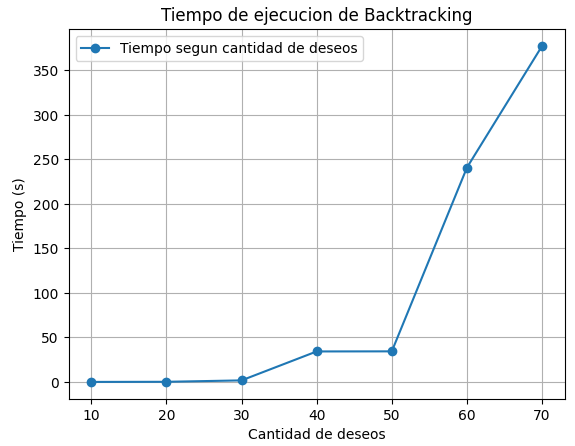
\includegraphics[width=0.7\textwidth]{img/tiempo_backtracking.png}

Podemos observar que, a medida que se va aumentando la cantidad de deseos, el tiempo de ejecución del algoritmo de Backtracking aumenta exponencialmente.
\end{center}

\begin{center}
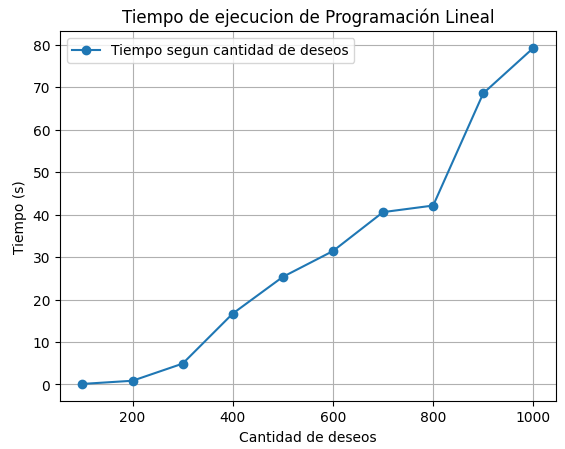
\includegraphics[width=0.7\textwidth]{img/tiempo_pl.png}

Podemos observar que, la curva con el algoritmo con Programación Lineal es más gradual que en comparación con la curva del algoritmo de Backtracking.
\end{center}

\begin{center}
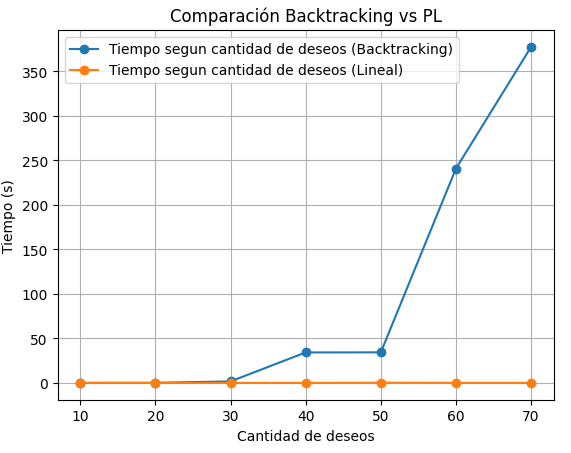
\includegraphics[width=0.7\textwidth]{img/backtracking_vs_pl.png}

Si comparamos los resultados de evaluar ambos algoritmos con los mismos sets de datos, observamos que el algoritmo de Programación Lineal se desempeña mejor que el algoritmo de Backtracking, el cual con pocos sets de datos aumenta exponencialmente sus tiempos de ejecución.
\end{center}

\begin{center}
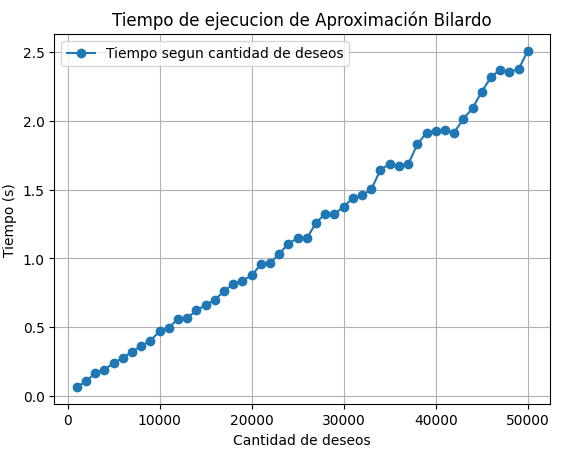
\includegraphics[width=0.7\textwidth]{img/tiempo_bilardo.png}

Se puede observar que el algoritmo de aproximación Bilardo reduce significativamente los tiempos de ejecución, a cambio de obtener una solución que puede diferir bastante con la solución óptima.
\end{center}

\begin{center}
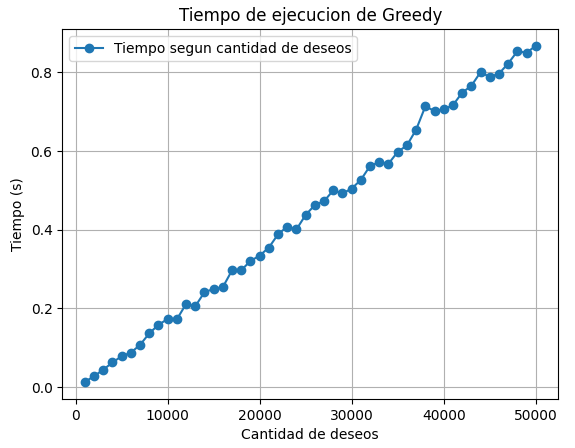
\includegraphics[width=0.7\textwidth]{img/tiempo_greedy.png}

También con este algoritmo de aproximación sucede que, se reduce significativamente el tiempo de ejecución a cambio de obtener una solución que puede diferir de la solución óptima.
\end{center}

\begin{center}
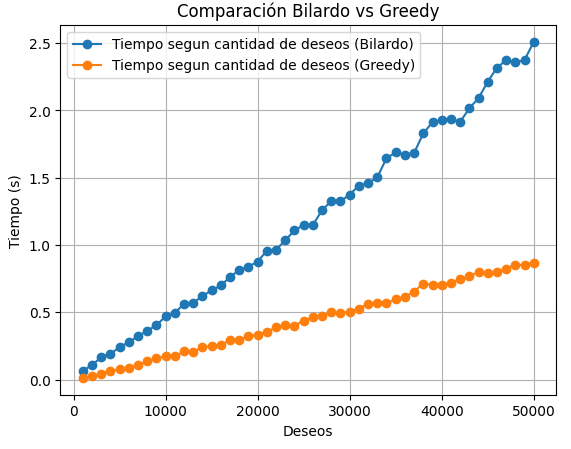
\includegraphics[width=0.7\textwidth]{img/bilardo_vs_greedy_1.png}

Podemos observar como los diferentes algoritmos de aproximación difieren en su complejidad, mostrando que el algoritmo Greedy tiene un tiempo de ejecución menor al algoritmo de Bilardo según la cantidad de deseos.
\end{center}

\begin{center}
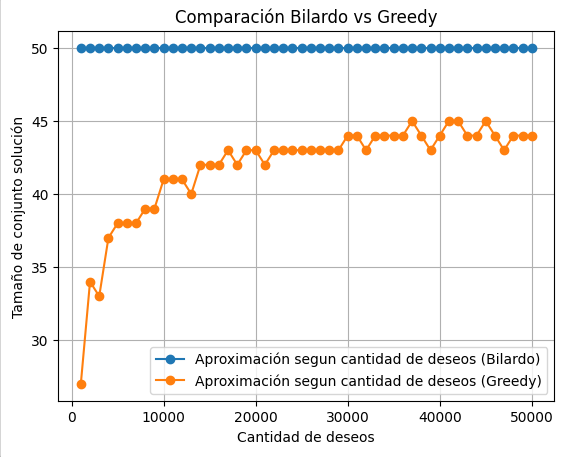
\includegraphics[width=0.7\textwidth]{img/bilardo_vs_greedy_2.png}

Vemos que el algoritmo de Bilardo siempre devuelve más jugadores según cantidad de deseos a comparación que el algoritmo Greedy, por lo tanto, pareciera ser mas óptimo este último.
\end{center}

\section{Conclusiones}

Podemos concluir que el algoritmo de Programación Lineal nos permitió encontrar una solución óptima evitando explorar un espacio exponencial de soluciones como se hace con el algoritmo de Backtracking, por lo cuál, gracias a esta metodología pudimos reducir significativamente los tiempos de ejecución del algoritmo.

También encontramos que el algoritmo de aproximación Greedy en promedio tiene mejor rendimiento que el algoritmo por aproximación Bilardo tanto en los tiempos de ejecución como hallando soluciones más próximas a la solución óptima.

Con grandes sets de datos, obtener la solución óptima requiere aumentar los tiempos de ejecución, por lo cuál, puede ser preferible utilizar un algoritmo de aproximación sabiendo que puede no obtener una solución óptima. 

\end{document}

\documentclass{article}
\usepackage{amsmath}
